% pagina op 1 zetten, begin van paper
\setcounter{page}{1}
\pagenumbering{arabic}
\chapter{Inleiding}
\label{ch:Inleiding}
Menselijke actieherkenning is het proces dat op een automatische manier (I) detecteert dat een persoon een bepaalde actie uitvoert en (II) herkennen welke actie dit is. 

Voorbeelden van zulke acties zijn lopen, stappen, zwaaien, springen, bukken, enz. Actieherkenning kent tal van toepassingen zoals fysiotherapie \cite{Deboeverie2016}, lichaamsanalyse \cite{Devi2015}, mens-robot interactie \cite{Li2018} en teleoperatie \cite{Ajili2017}. In deze masterproef wordt actieherkenning gecombineerd met teleoperatie, meer specifiek voor rijdende voorwerpen, zoals een robot of een slimme fiets. Een operator kan dan door enkel gebaren uit te voeren het voorwerp besturen. Belangrijk hierbij is het real-time aspect; een te trage herkenning van de actie zorgt voor een late reactie waardoor er potentieel ongevallen kunnen plaatsvinden. 

\section{Probleemstelling}
Men is reeds in staat om voor zowel kleurenbeelden als dieptebeelden actieherkenning toe te passen op een betrouwbare manier. Echter blijft het moeilijk om dit te realiseren in een real-time scenario, waarbij snelle beslissingen gemaakt moeten worden. Een groot probleem is de onzekerheid van de actie. 

In de literatuur worden er vaak methoden (\cite{Xia2012}, ...) beschreven die acties herkennen op video's waarop slechts één actie uitgevoerd wordt. De actielabel wordt ook maar nadien toegekend, als de video reeds gedaan is. Een betere aanpak zou de actielabel toekennen op het moment dat de actie bezig is, op een video waarbij meerdere acties kunnen uitgevoerd worden op hetzelfde moment. In de literatuur worden dit \textit{untrimmed video's} genoemd. In zulke video's zijn de actielabels, actiepositie en actieduur onbekende parameters.

De THUMOS Challenge \footnote{\url{http://www.thumos.info}} werd georganiseerd in 2015 en was een initiatief om op een competitieve manier het probleem van actieherkenning in untrimmed video's te onderzoeken. Ze bieden een dataset aan met untrimmed video's die scenario's uit het echte leven bevatten.

Het doel van deze masterproef is om eerst te onderzoeken welke methoden er al bestaan op vlak van actieherkenning in untrimmed video's en hoe deze geoptimaliseerd kunnen worden zodat ze efficiënt werken op de skeletdata van een Kinect. In hoofdstuk \ref{ch:methodologie} wordt de uitwerking beschreven.


\section{De Kinect}
De Kinect (figuur \ref{fig:KinectSensorVersies}) werd initieel ontworpen voor gebruik met de Xbox 360.  als een manier om de gebruiker zelf als spelcontroller te beschouwen. Dit is een grote vordering in vergelijking met bijvoorbeeld de Wii Remote, waarbij de gebruiker een controller moet hebben om acties uit te voeren. Door de combinatie van de diepte- en kleurenbeelden die de Kinect kan leveren kunnen er skeletbeelden gegenereerd worden. Voor elke frame kan de Kinect tot maximaal 25 skeletjoints genereren, voor maximaal zes personen, die drie-dimensionale coördinaten voorstellen van voornamelijk gewrichten van het lichaam. Voorbeelden van locaties waarop joints komen zijn onder andere het hoofd, de schouders, de ellebogen, de polsen, enz. Dit heeft een groot voordeel: het detecteren van de low-level features uit de kleuren- en dieptebeelden om de skeletjoints te bepalen wordt overgelaten aan de Kinect zelf. Sinds de opkomst van de Kinect is het onderzoek naar actieherkenning met behulp van skeletjoints weer op gang geschoten \cite{Deboeverie2016}, \cite{Xia2012}, \cite{Wang2014},\cite{Vemulapalli2014}, \cite{Li2018}.

Ondanks het succes van de Kinect heeft Microsoft toch besloten om het product niet meer als entertainmentproduct te verkopen, maar wel als een tool die onderzoekers en ontwikkelaars kunnen helpen. Daarom laten ze de oude Kinect achterwegen en maken ze een nieuwe versie  die de  naam \textit{Azure Kinect} draagt. Deze Kinect is rechtstreeks verbonden met het Azure platform van Microsoft. In deze masterproef wordt de tweede versie van de Kinect gebruikt (figuur \ref{fig:KinectSensorOne}).

\begin{figure}
	\begin{subfigure}[t]{0.48\textwidth}
		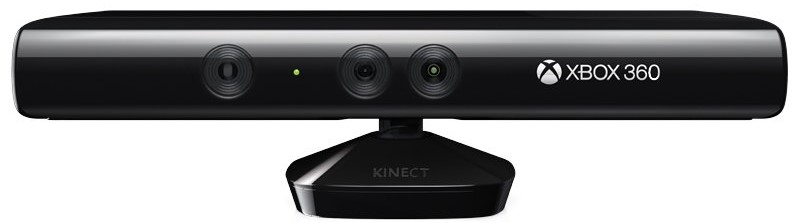
\includegraphics[width=\linewidth]{KinectSensor360}
		\caption{De originele Kinect sensor, ontwikkeld int 2010 voor de Xbox 360.}
	\end{subfigure}
	\begin{subfigure}[t]{0.48\textwidth}
		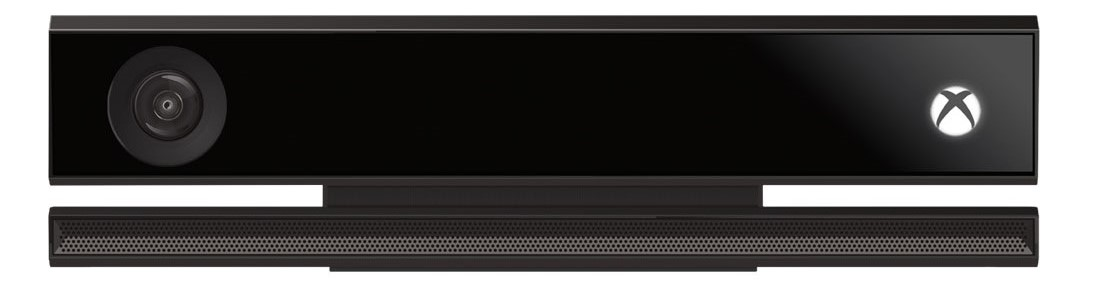
\includegraphics[width=\linewidth]{KinectSensorOne}
		\caption{De tweede iteratie van de Kinect sensor, specifiek gemaakt voor Xbox One en uitgebracht in 2013.}
		\label{fig:KinectSensorOne}
	\end{subfigure}
	\caption{Twee versies van de Kinect sensor.}
	\label{fig:KinectSensorVersies}
\end{figure}

\section{Structuur}
In hoofdstuk \ref{ch:methodologie} wordt de algemene methodologie beschreven die gebruikt wordt om deze masterproef te realiseren, waarom deze gebruikt wordt en wat het beoogde eindresultaat is. Verder wordt er in hoofdstuk \ref{ch:features} en hoofdstuk \ref{ch:classificatie} een overzicht gegeven van bestaande methoden en welke features en classifiers zij gebruiken. In hoofdstuk \todo{hoofdstuk uitwerking, resultaten, conclusie}
